\documentclass{beamer}
\usetheme{Boadilla}

\usepackage{algorithm2e}
\usepackage{amsmath}
\usepackage{amsfonts}
\usepackage{hyperref}

\usepackage{amsmath}
\DeclareMathOperator*{\argmax}{arg\,max}
\DeclareMathOperator*{\argmin}{arg\,min}


\title{Super-Resolution Neural Operator}
\author{Parviz Karimov}
\institute{MIPT, 2024}


\begin{document}

\begin{frame}
    \titlepage
\end{frame}


\begin{frame}
    \tableofcontents
\end{frame}


\section{Motivation}

\begin{frame}{Motivation}
    \begin{block}{}
     Most DNNs are developed in the configuration of single scaling factors, which cannot be used in scenarios requiring arbitrary SR factors. Recently, implicit neural functions (INF) have been proposed to represent images in arbitrary resolution, and paving a feasible way for continuous SR. To share knowledge across instances instead of fitting individual functions for each signal, encoder-based methods are proposed to retrieve latent codes for each signal, and then a decoding MLP is shared by all the instances to generate the required output, where both the coordinates and the corresponding latent codes are taken as input. However, the point-wise behavior of MLP in the spatial dimensions results in limited performance when decoding various objects, particularly for high-frequency components
    \end{block} 
\end{frame}

\section{General Problem Statement}
\begin{frame}{Problem Statement}
    \begin{block}{}
        Consider the following PDE:
        $$
        (L_au)(x) = f(x), x \in D
        $$
        $$
        u(x) = 0, x \in \partial D,
        $$
        where $u : D \rightarrow \mathbb{R}^{d_u}$ is the solution function residing in the Banach space $\mathcal{U}$, and $L: \mathcal{A} \rightarrow L(\mathcal{U}, \mathcal{U}^*)$ is an operator-valued functional that maps the coefficient function $a \in \mathcal{A}$ of the PDE to $f \in \mathcal{U}^*$.

        Neural operator (NO) seeks a feasible operator $\mathcal{G} : \mathcal{A} \rightarrow \mathcal{U}, a \mapsto u$, directly mapping the coefficient to the solution within an acceptable tolerance.
    \end{block}

    \begin{block}{}
        The infinitely dimensional operator learning problem $\mathcal{G} \leftarrow \mathcal{G}_{\theta}$ is associated with the empirical-risk minimization problem.
        $$
        \min_\theta \mathbb{E}_{a \sim \mu} ||\mathcal{G}(a) - \mathcal{G}_\theta(a)||_{\mathcal{U}} \approx \min_{\theta} \frac{1}{N} \sum_j ||u^{(j)} - \mathcal{G}_\theta(a^{(j)})||_{\mathcal{U}}
        $$

        % If $\mathcal{A}$ is defined on the bounded domain $D \subset \mathbb{R}^d$ inputs and outputs are vector-valued functions with dimension $d_z$, then $\mathcal{G}_\theta$ can be formulated as follows:
        % $$
        % $$
    \end{block}

\end{frame}

\begin{section}{SRNO}
    \begin{frame}{SRNO Problem Statement}
    \begin{block}{}
        Let $(\mathcal{H},\langle\cdot,\cdot\rangle_{\mathcal{H}})$ be a Hilbert space equipped with the inner-product structure, which is continuously embedded in the space of continuous functions $C^0(\Omega)$, with $\Omega \subset \mathbb{R}^2$ a bounded domain. An image is defined as a vector-valued function $\mathcal{H}\ni f:\Omega \rightarrow \mathbb{R}^3$. Assume we can access the function values of $f$ at the coordinates $\{x_i\}_{i=1}^{n_h} \subset \Omega$ with the biggest discretization size $h$.
    \end{block}

    \begin{block}{}
        The goal is to learn a super-resolution neural operator between two Hilbert spaces with different resolutions: $\mathcal{S}_{\theta}: \mathcal{H}\supset\mathcal{H}(\Omega_{h_c}) \rightarrow \mathcal{H}(\Omega_{h_f})\subset\mathcal{H}$, where $h_c,h_f$ denotes the coarse and the fine grid sizes, respectively. Given $N$ function pairs $\{a^{(k)},u^{(k)}\}_{k=1}^N$, where $a^{(k)}\in\mathcal{H}(\Omega_{h_c})$ and $u^{(k)}\in\mathcal{H}(\Omega_{h_f})$. SRNO parameterized by $\theta$ can be solved through the associated empirical-risk minimization problem:
        $$
        \min_{\theta}\frac{1}{N}\sum_{k=1}^N{\lVert u_{h_f}^{(k)}-\mathcal{S}_{\theta}(a_{h_c}^{(k)}) \rVert_{\mathcal{H}}.}
        $$
    \end{block}
    \end{frame}

    \begin{frame}{Overview}
    \begin{figure}[H]
        \centering
        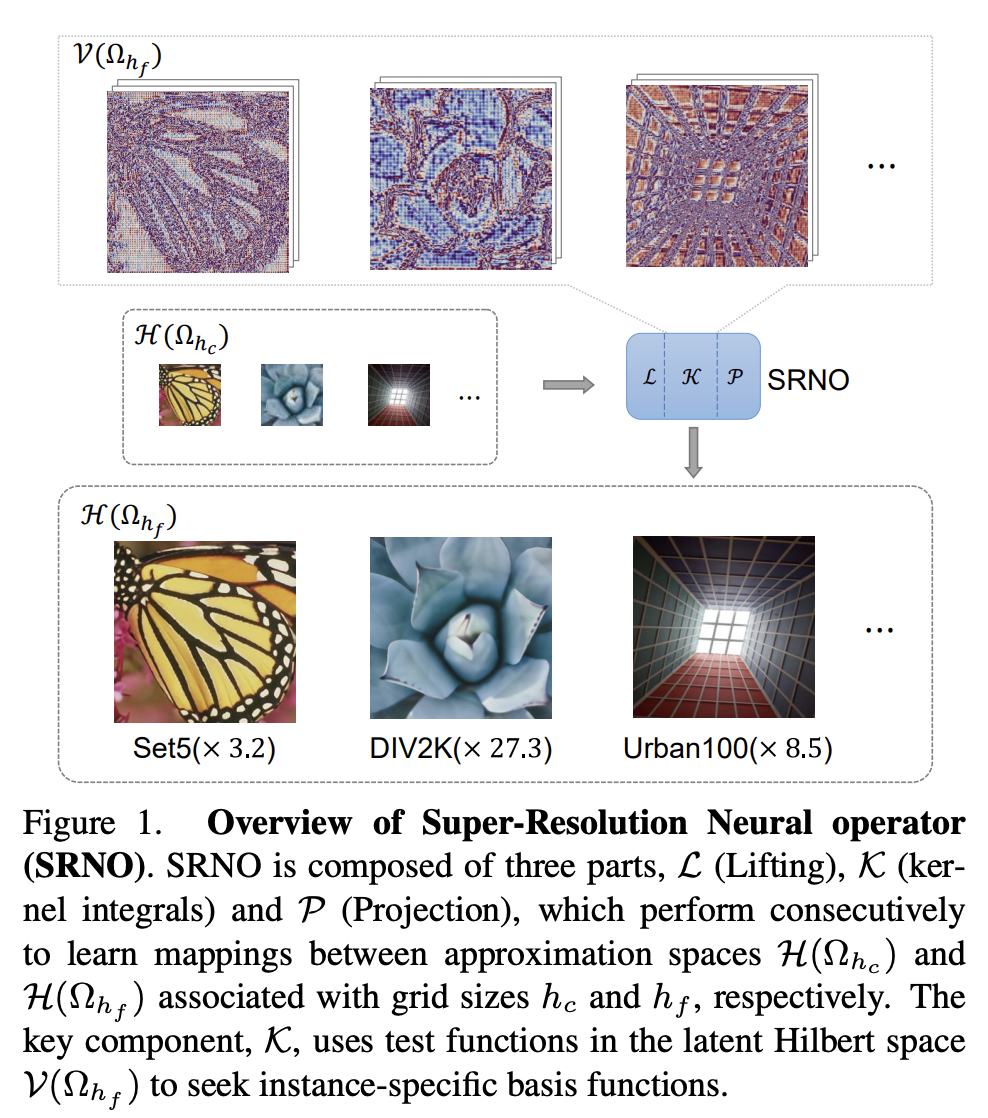
\includegraphics[width=0.5\linewidth]{2.png}
        \label{fig:Overview of Super-Resolution Neural Operator}
    \end{figure}
        
    \end{frame}

    \begin{frame}{Overview}
    \begin{figure}[H]
        \centering
        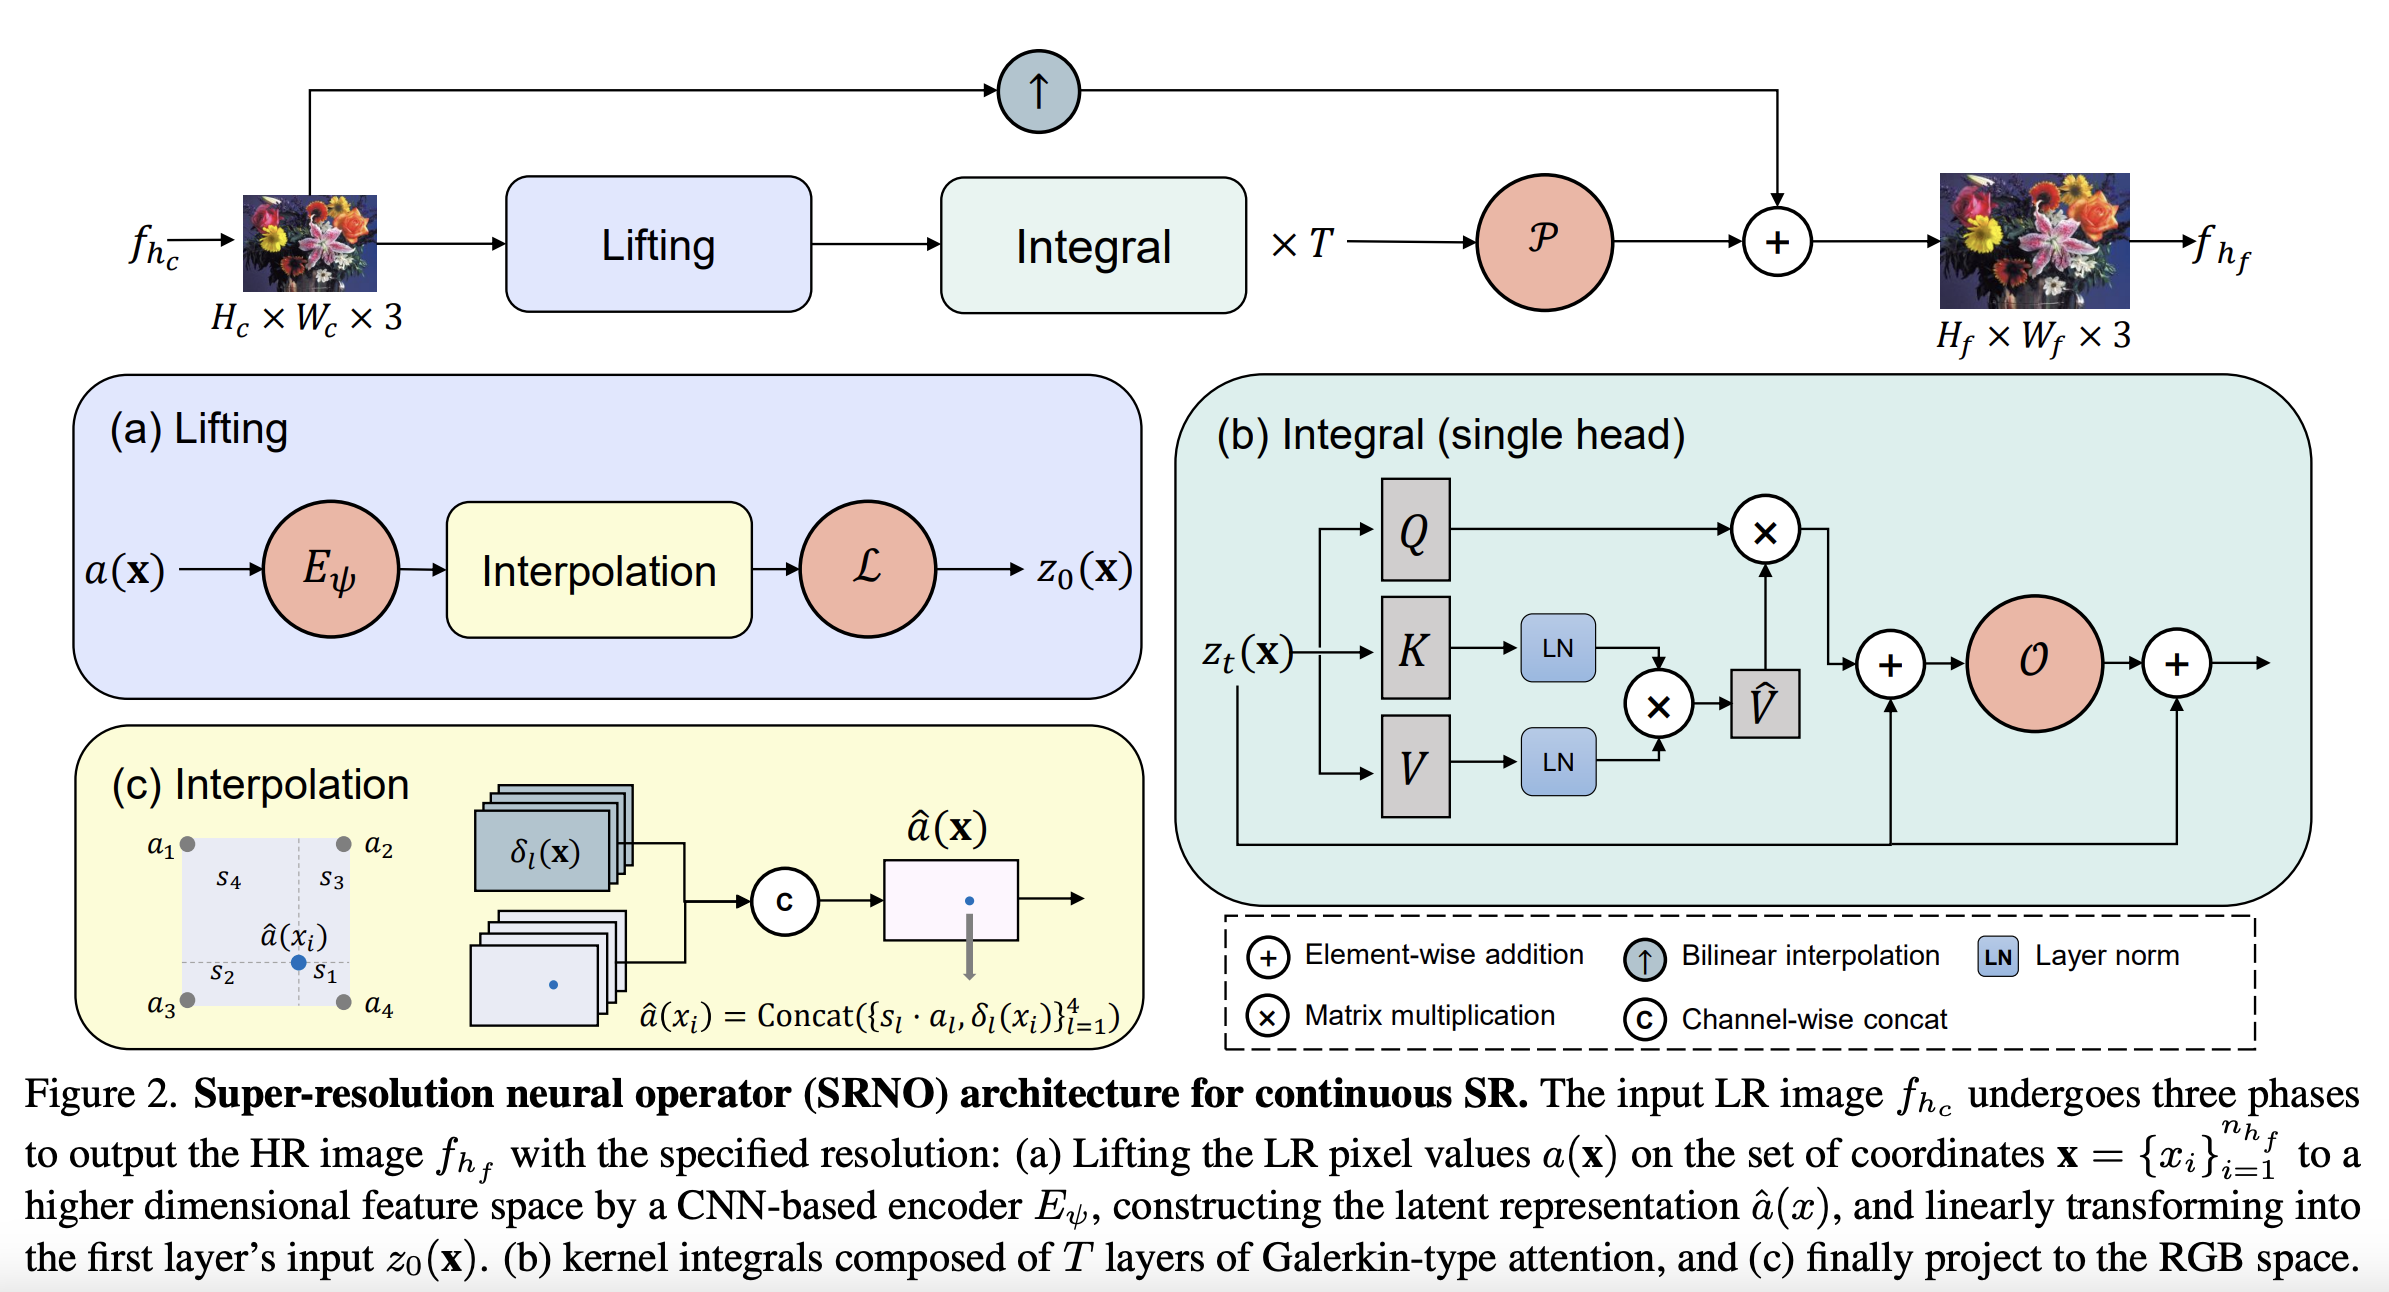
\includegraphics[width=\linewidth]{1.png}
        \label{fig:SRNO architecture}
    \end{figure}
        
    \end{frame}

    \begin{frame}{Overview}
    \begin{block}{}
    As a whole, the process of getting HR image as a result of SRNO is the following:
    \begin{align*}
 z_0(x) &= \mathcal{L}(x,a(x)), \label{lifing}  \\
 z_{t+1}(x) &= z_t(x)+\mathcal{O}((\mathcal{K}_t(z_t))(x) + z_t(x)),\label{iterative} \\
 u(x) &= \mathcal{P}(z_T(x)),
    \end{align*}
    
    where $\mathcal{L}: \mathbb{R}^{d_a+d} \rightarrow \mathbb{R}^{d_z}$, and $\mathcal{P}: \mathbb{R}^{d_z} \rightarrow \mathbb{R}^{d_u}$ are the local lifting and projection functions respectively , mapping the input $a$ to its first layer hidden representation $z_0$ and the last layer hidden representation $z_T$ back to the output function $u$. $W: \mathbb{R}^{d_z} \rightarrow \mathbb{R}^{d_z}$ is a point-wise linear transformation, and $ \sigma: \mathbb{R}^{d_z} \rightarrow \mathbb{R}^{d_z}$ is the nonlinear activation function.

    \end{block}
        
    \end{frame}

\end{section}

\begin{section}{Results}
    \begin{frame}{Quantitative Results}

    \begin{table*}
    \centering
    \scalebox{0.7}{
    \begin{tabular}{c|ccc|ccccc}
        \multirow{Method} & \multicolumn{3}{c|}{In-distribution} & \multicolumn{5}{c}{Out-of-distribution} \\
        & $\times$2 & $\times$3 & $\times$4 & $\times$6 & $\times$12 & $\times$18 & $\times$24 & $\times$30 \\
        \hline
        Bicubic & 31.01 & 28.22 & 26.66 & 24.82 & 22.27 & 21.00 & 20.19 & 19.59 \\
        EDSR-baseline & 34.55 & 30.90 & 28.94 & - & - & - & - & - \\
        EDSR-baseline-MetaSR & 34.64 & 30.93 & 28.92 & 26.61 & 23.55 & 22.03 & 21.06 & 20.37 \\
        EDSR-baseline-LIIF & 34.67 & 30.96 & 29.00 &
        26.75 & 23.71 & 22.17 & 21.18 & 20.48 \\
        EDSR-baseline-LTE & 34.72 & 31.02 & 29.04 &
        26.81 & 23.78 & 22.23 & 21.24 & 20.53 \\
        EDSR-baseline-SRNO (ours) & \textbf{34.85} & \textbf{31.11} & \textbf{29.16} &
        \textbf{26.90} & \textbf{23.84} & \textbf{22.29} & \textbf{21.27} & \textbf{20.56} \\
        \hline
        RDN-MetaSR & 35.00 & 31.27 & 29.25 & 26.88 & 23.73 & 22.18 & 21.17 & 20.47 \\
        RDN-LIIF & 34.99 & 31.26 & 29.27 & 26.99 & 23.89 & 22.34 & 21.31 & 20.59 \\
        RDN-LTE & 35.04 & 31.32 & 29.33 & 27.04 & 23.95 & 22.40 & 21.36 & 20.64 \\
        RDN-SRNO (ours) & \textbf{35.16} & \textbf{31.42} & \textbf{29.42} &
        \textbf{27.12} & \textbf{24.03} & \textbf{22.46} & \textbf{21.41} & \textbf{20.68} \\
    \end{tabular}}
    \caption{\footnotesize\textbf{Quantitative comparison on DIV2K validation set (PSNR (dB))}. The best performance are bolded. EDSR-baseline trains separate models for the three in-distribution scales. The rest methods use a single model for all scales, and are trained with continuous random scales uniformly sampled in $\times1$--$\times4$.}
    \label{tab:1}
    %\vspace{-0.5em}
    \end{table*}
        
    \end{frame}

    \begin{frame}{Qualititative Results}
    \begin{figure}
        \centering
        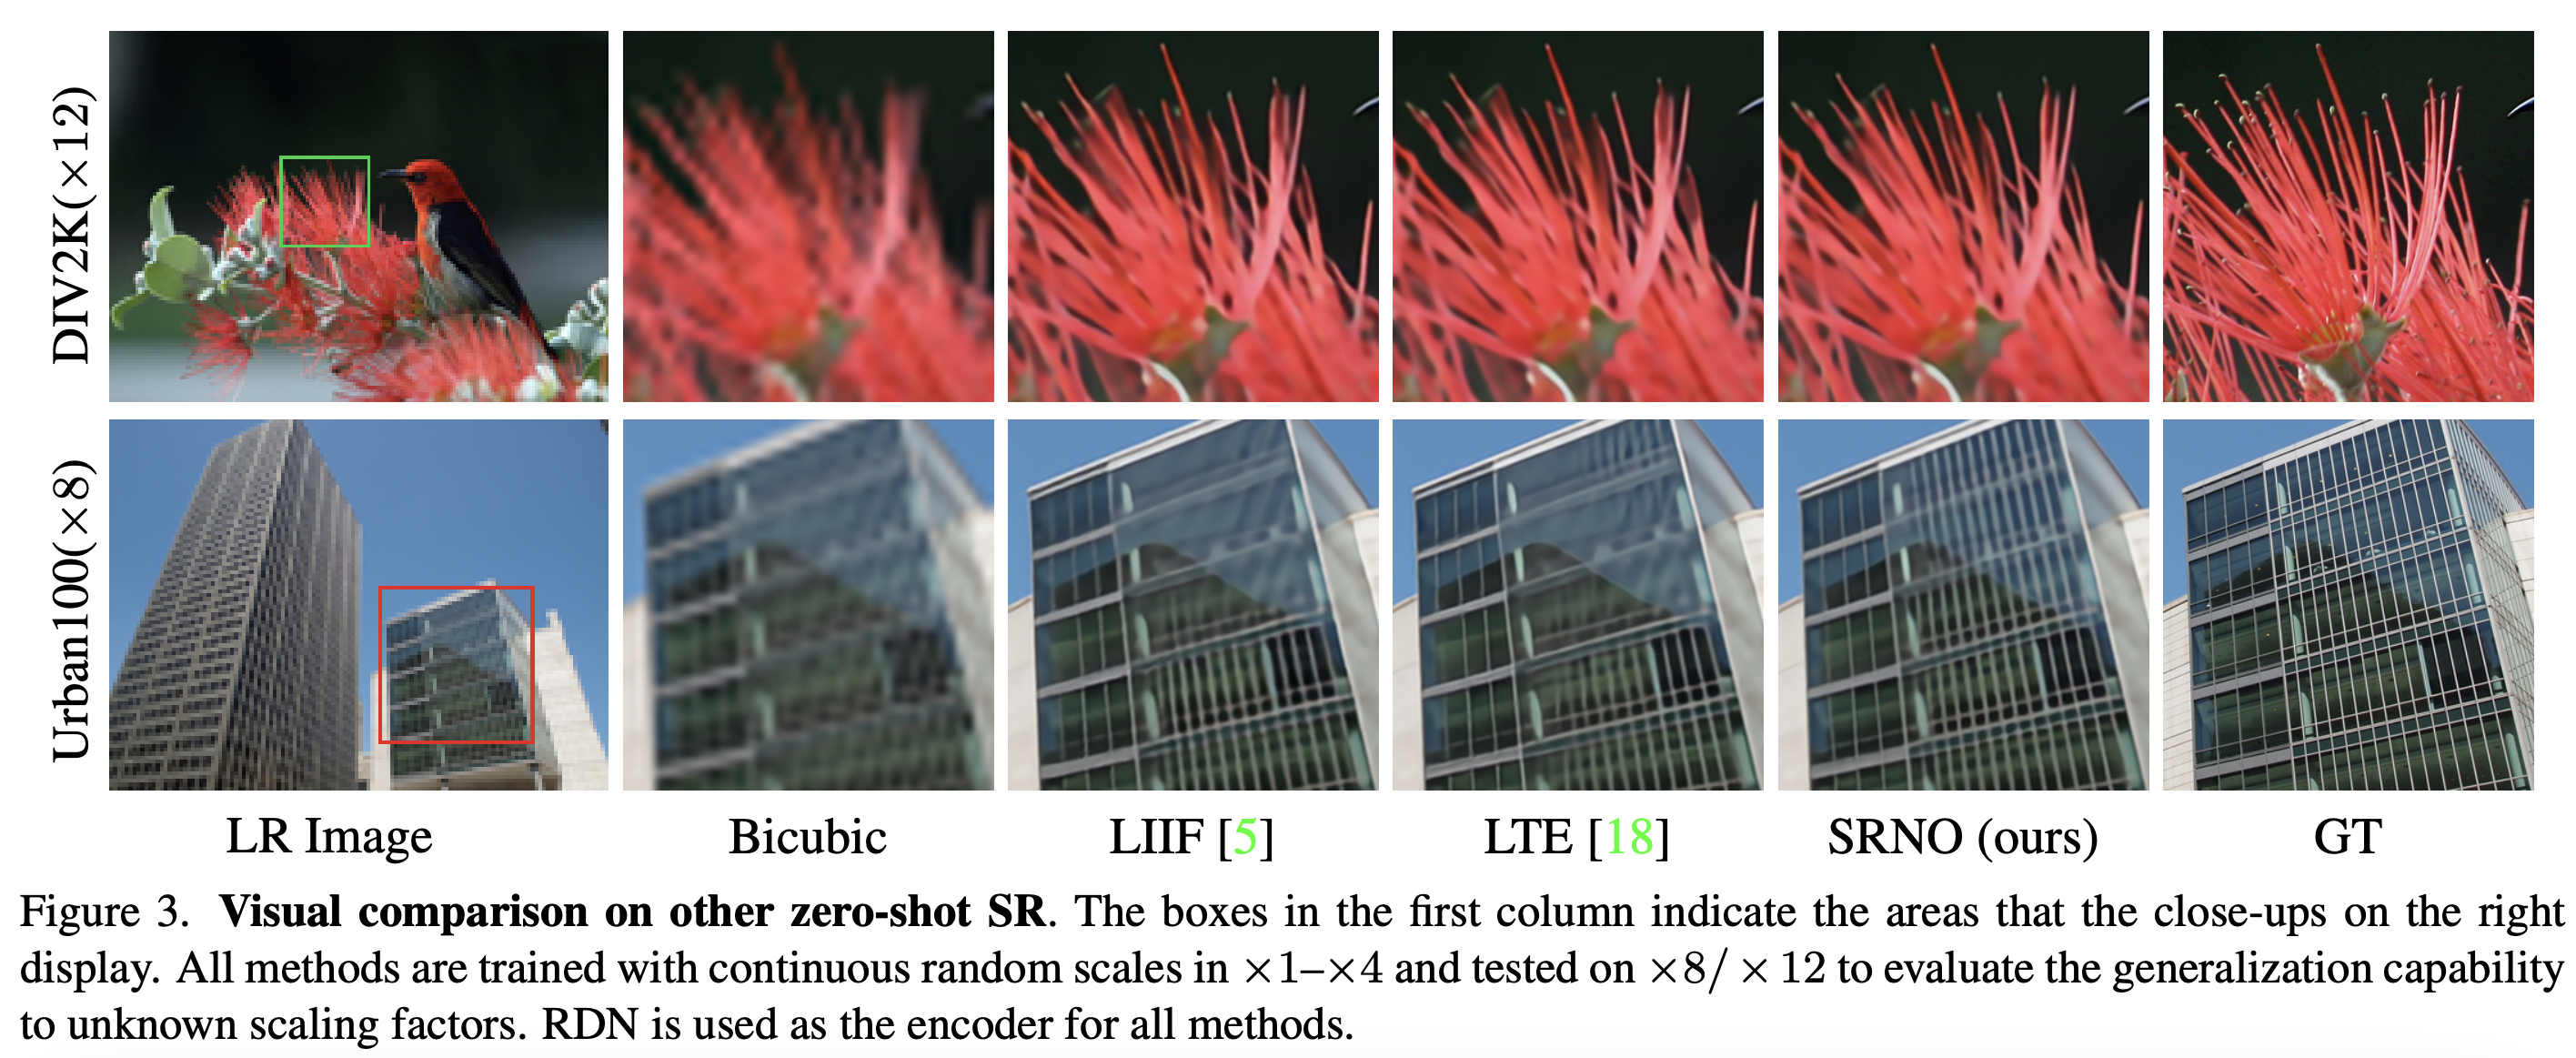
\includegraphics[width=\linewidth]{3.png}
    \end{figure}
    \end{frame}

    \begin{frame}{Qualititative Results}
    \begin{figure}
        \centering
        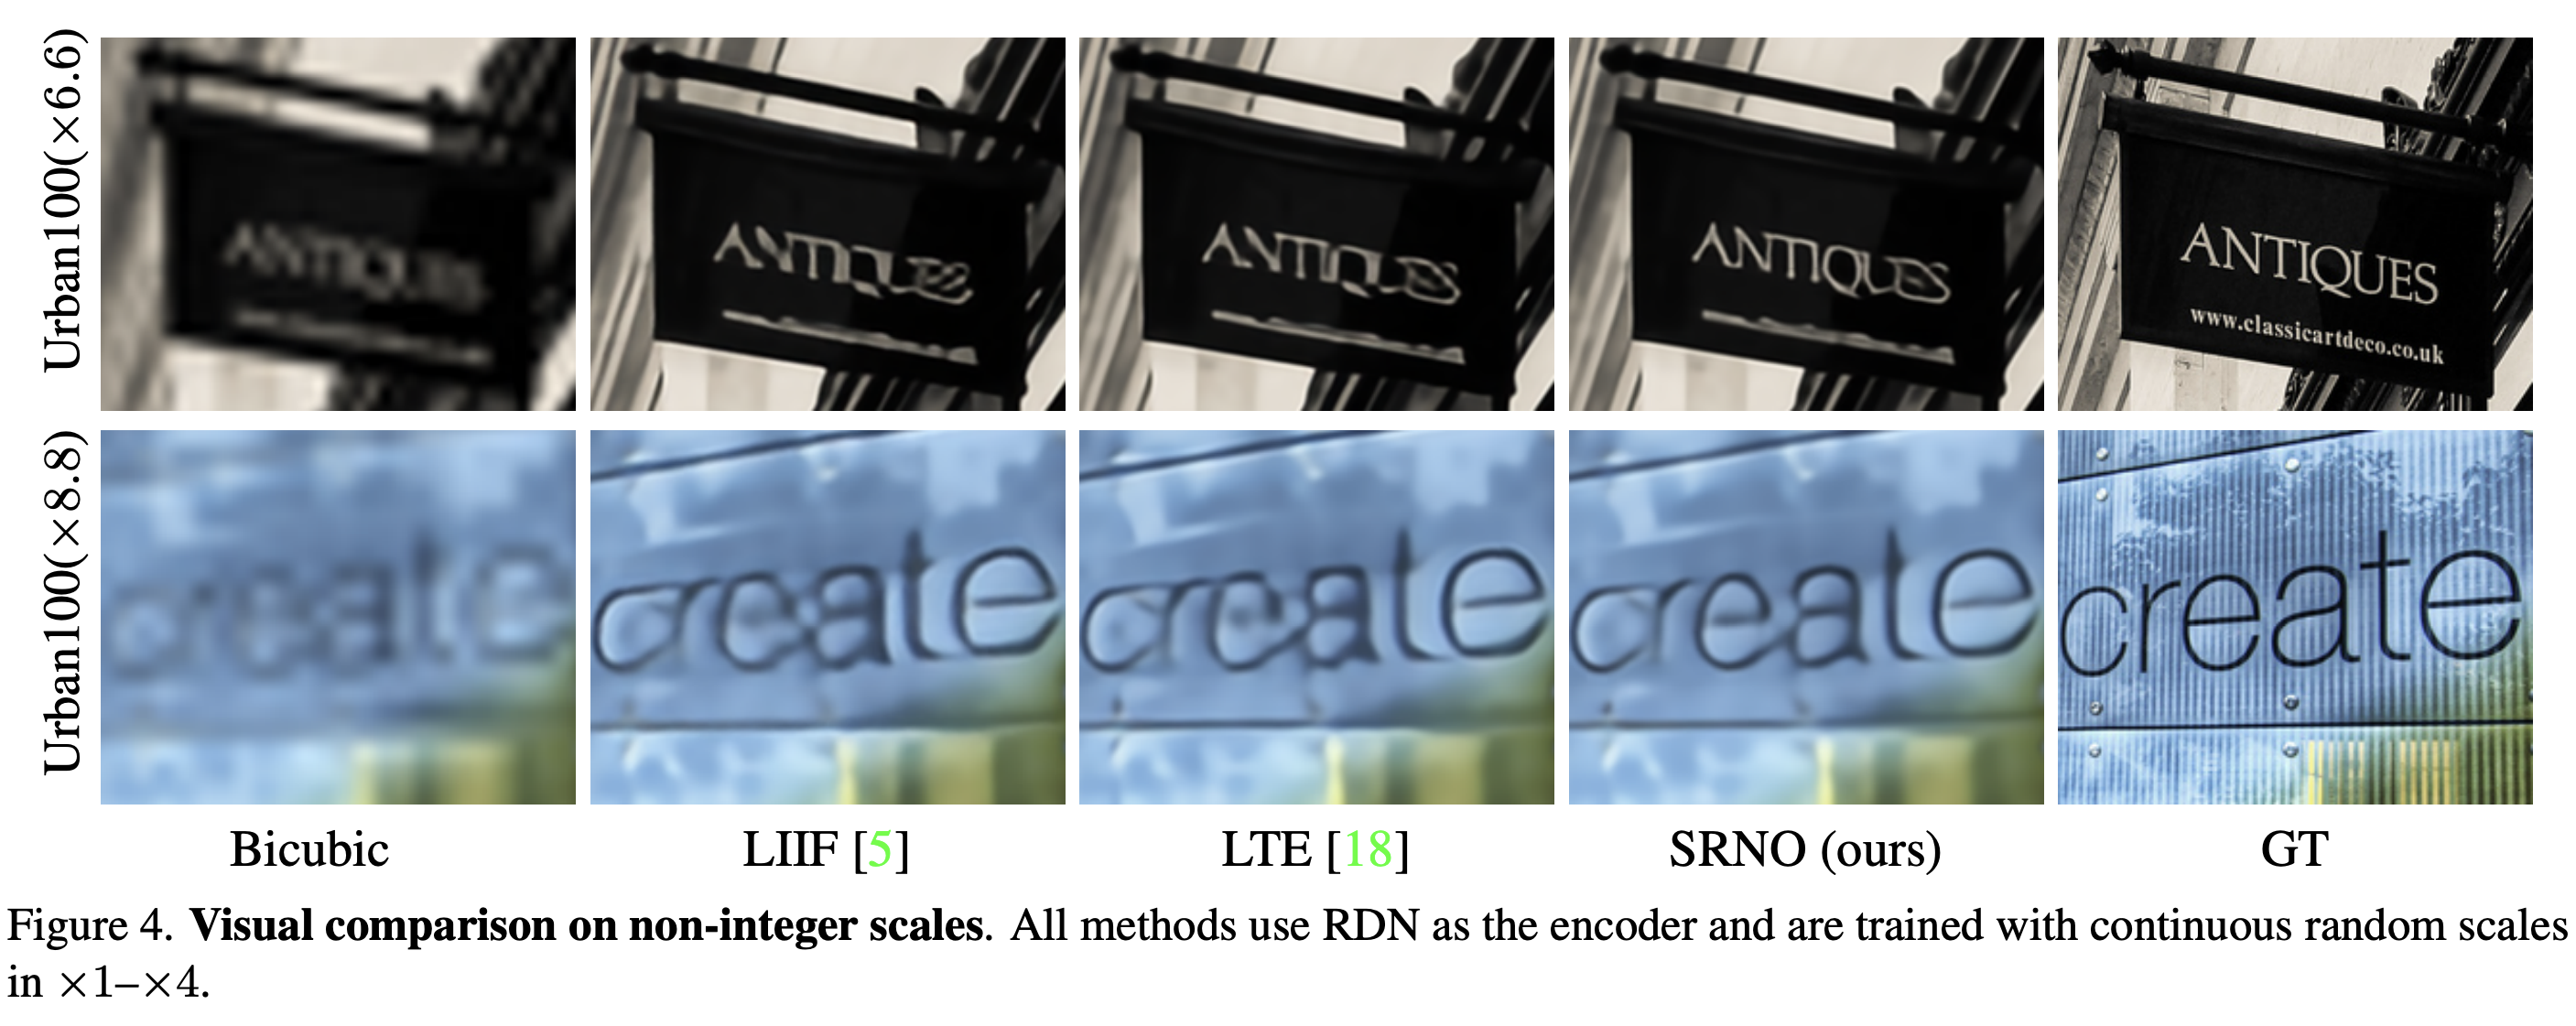
\includegraphics[width=\linewidth]{4.png}
    \end{figure}
    \end{frame}
\end{section}

\begin{frame}{Literature}
    \begin{enumerate}
        \item \textbf{Main article} \href{https://openaccess.thecvf.com/content/CVPR2023/papers/Wei_Super-Resolution_Neural_Operator_CVPR_2023_paper.pdf}
        {Super-Resolution Neural Operator}.
    \end{enumerate}
\end{frame}



\end{document}